\documentclass[11pt]{article}
 
\usepackage[margin=.95in]{geometry} 
\usepackage{amsmath,amsthm,amssymb, graphicx, multicol, array}
 
\newcommand{\N}{\mathbb{N}}
\newcommand{\Z}{\mathbb{Z}}
 

\begin{document}
 
\title{Homework 5}
\author{Juliette Franqueville\\
}
\maketitle

\subsection*{(1) (a)}


\begin{figure}[!h]
    \centering
    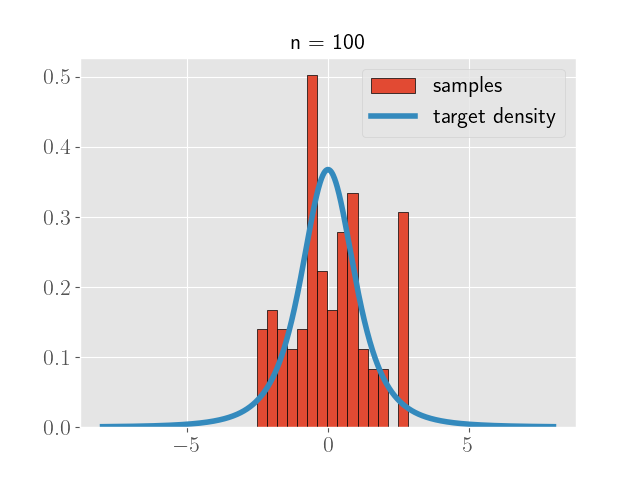
\includegraphics[scale=.5
    ]{../figures/resamples_n_100.png}
    \caption{samples and t distribution for $n=100$}
    \label{fig:my_label}
\end{figure}

\begin{figure}[!h]
    \centering
    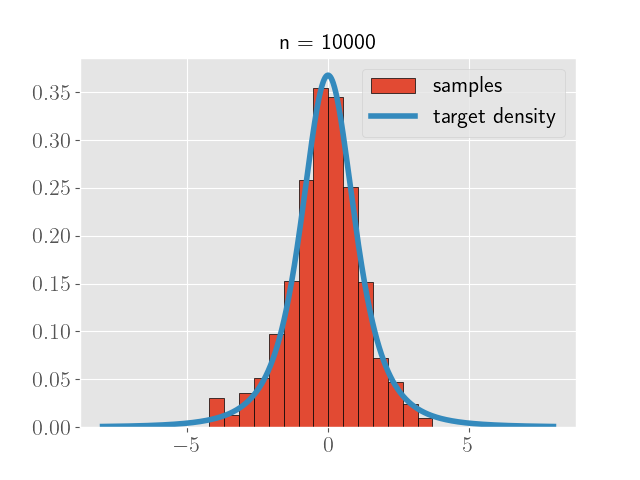
\includegraphics[scale=.5
    ]{../figures/resamples_n_10000.png}
    \caption{samples and t distribution for $n=10,000$}
    \label{fig:my_label}
\end{figure}
\newpage

\subsection*{(b)}
For $n=100$, the estimated mean and variance were 0.12 and 0.84, respectively. For $n=10,000$, they were 0.03 and 1.67. The means were close to the actual mean (0), but the variances were underestimated compared to the actual variance of $t_3$ (3). This is not surprising because the tails of the normal are not as wide as those of the $t$ distribution. In other words, the normal distribution does not fully cover the $t$ distribution, so the points far from the mean in the tails do not get sampled, which makes the variance too small. I redid this exercise with a uniform distribution that  covered $t_3$ better, and the variances were closer to 3.

\subsection*{(2)}
\begin{align*}
    (X_1|X_2) & \propto (X_1, X_2)\\
    & \propto (1-\rho^2)^{-1/2}\text{exp} \left( -\frac{1}{2(1-\rho^2)} \begin{bmatrix} x_1-\mu_1, &x_2-\mu_2 \end{bmatrix} \begin{bmatrix} 1 & -\rho \\ -\rho & 1 \end{bmatrix}\begin{bmatrix} x_1-\mu_1 \\ x_2-\mu_2 \end{bmatrix}\right)\\
    & \propto (1-\rho^2)^{-1/2}\text{exp} \left( -\frac{1}{2(1-\rho^2)}[(x_1-\mu_1)^2-2\rho(x_1-\mu_1)(x_2-\mu_2) + (x_2-\mu_2)^2] \right)\\
     & \propto (1-\rho^2)^{-1/2}\text{exp} \left( -\frac{1}{2(1-\rho^2)}[x_1^2-2x_1(\mu_1+\rho x_2 - \rho x_1)] \right)\\
     & \propto \mathcal{N}(\mu_1 + \rho(x_2-x_1), 1-\rho^2)
\end{align*}

To get $(X_2|X_1)$, we simply swap $X_1$ ad $X_2$. We then use a Gibbs sampler to produce the following plots. I set burn in $=500$ and thin every 2 iterations.

\begin{figure}[!h]
    \centering
    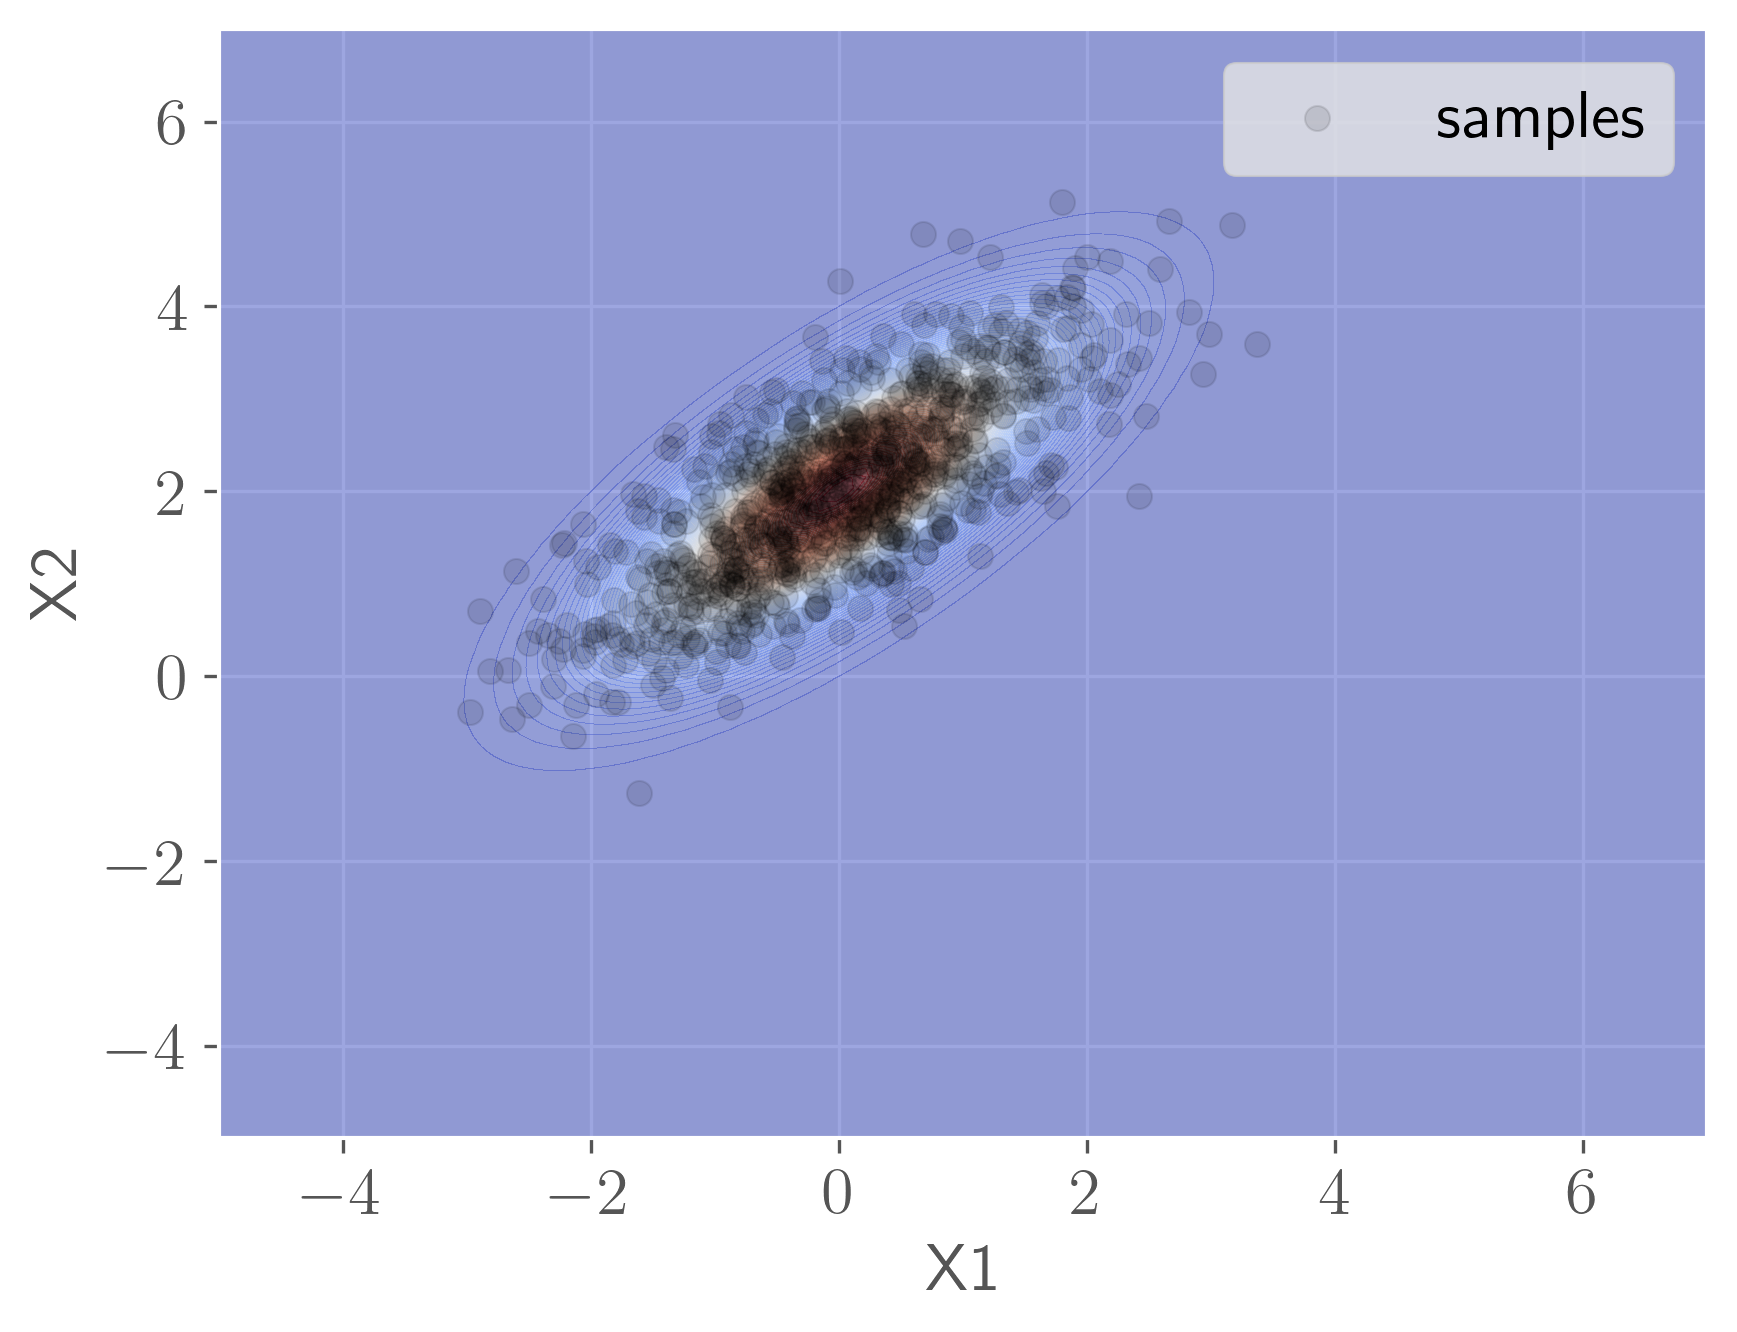
\includegraphics[scale=.6
    ]{../figures/bivar.png}
    \caption{samples and true distribution}
    \label{fig:my_label}
\end{figure}

\begin{figure}[!h]
    \centering
    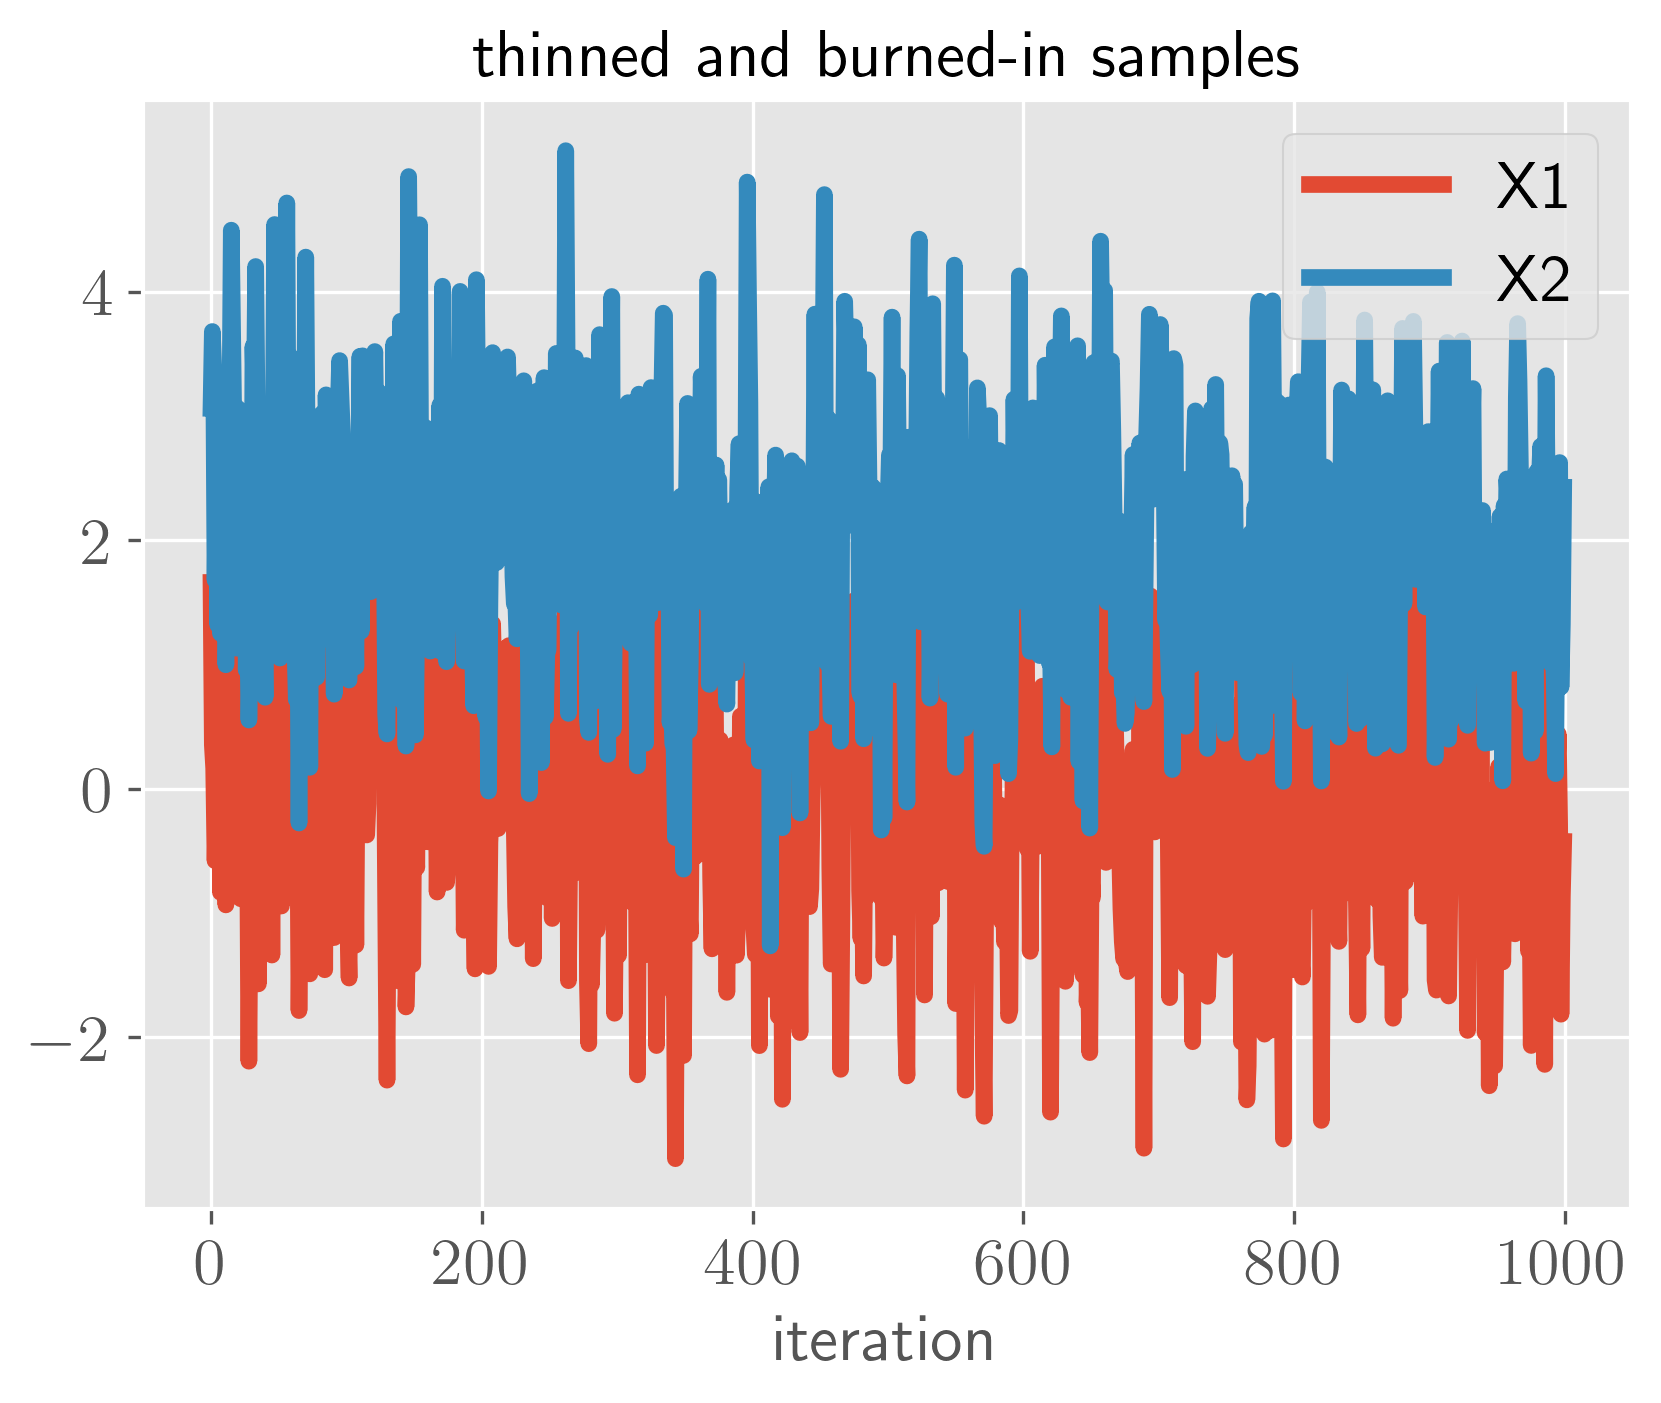
\includegraphics[scale=.6
    ]{../figures/traces.png}
    \caption{Traces}
    \label{fig:my_label}
\end{figure}

\begin{figure}[!h]
    \centering
    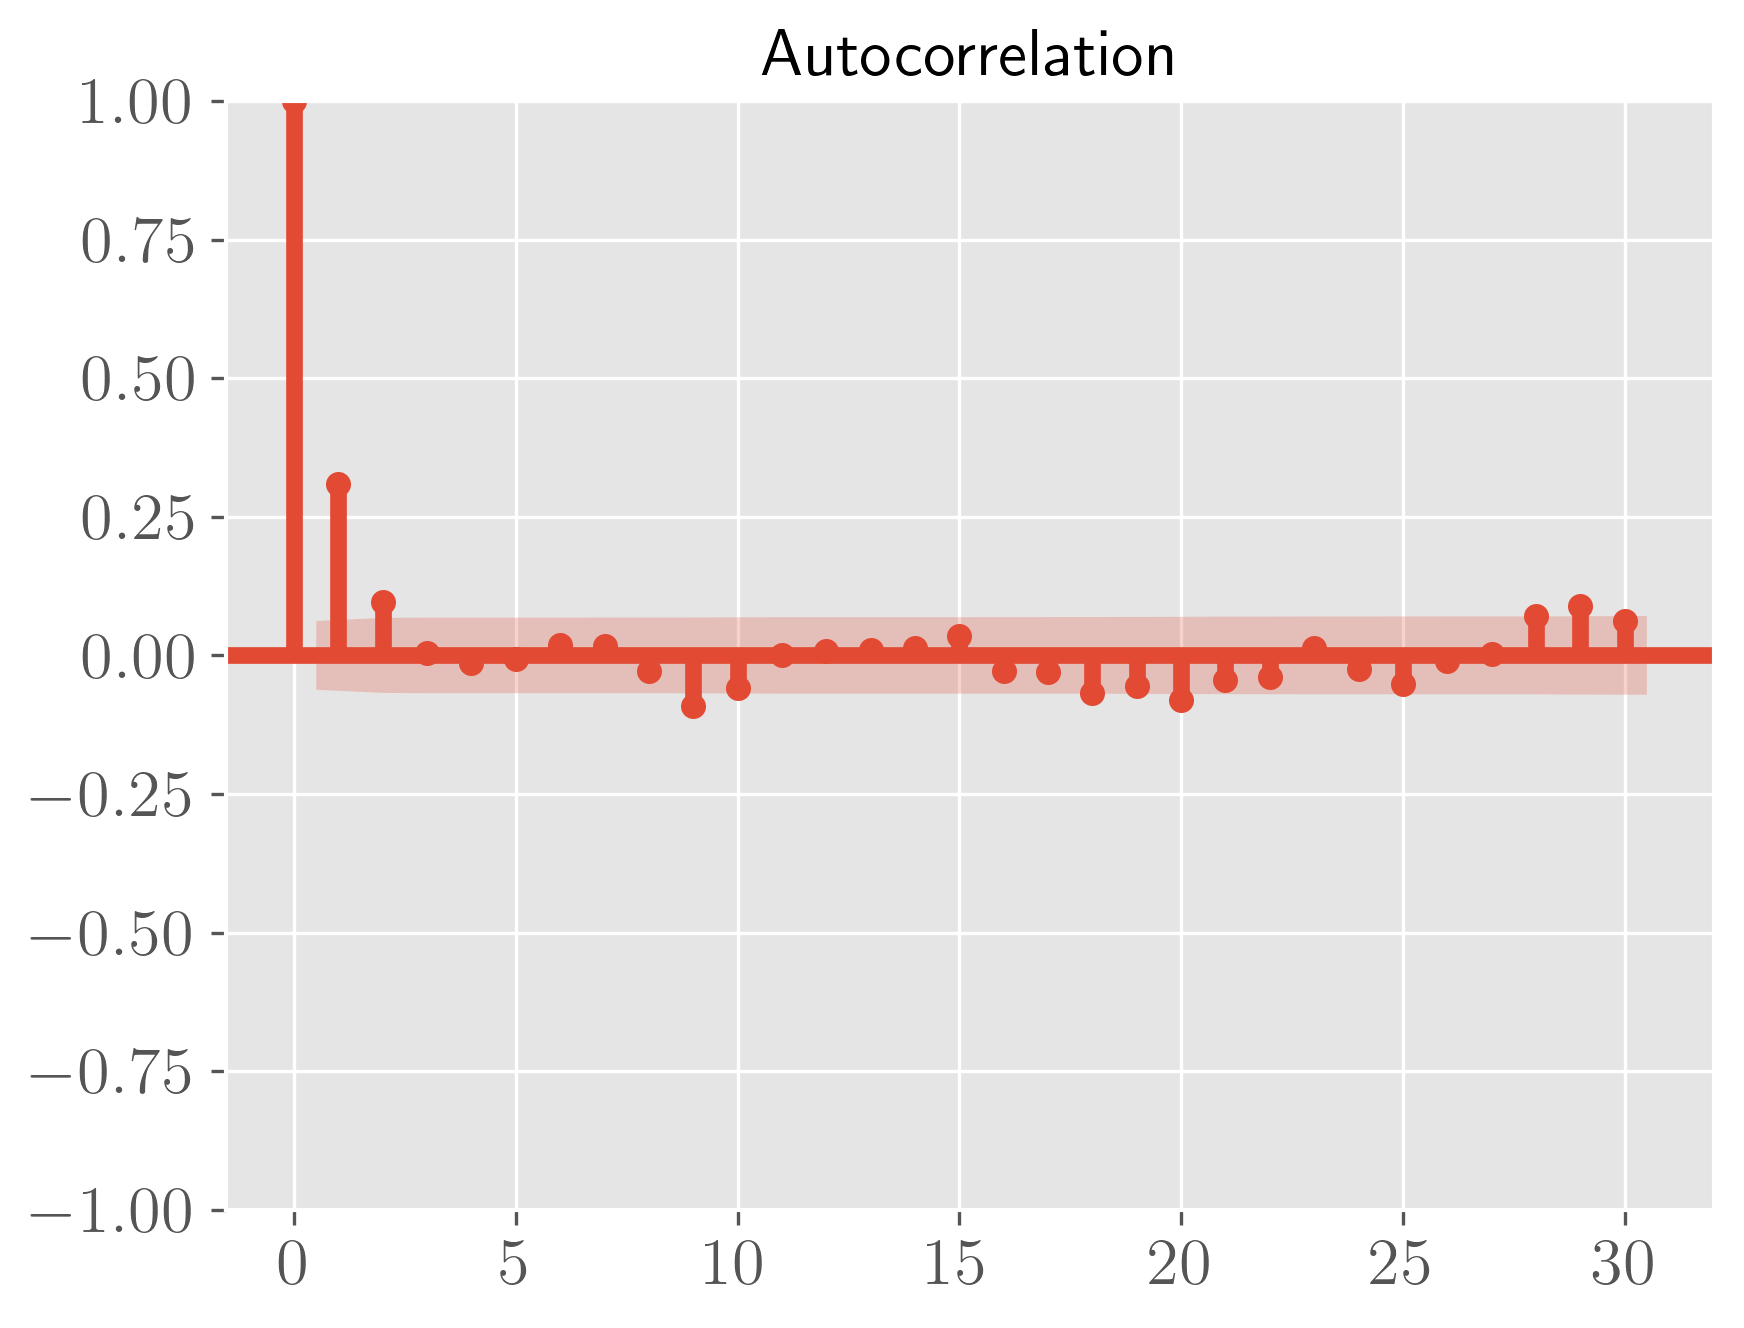
\includegraphics[scale=.6
    ]{../figures/acf1.png}
    \caption{ACF for $X_1$}
    \label{fig:my_label}
\end{figure}

\begin{figure}[!h]
    \centering
    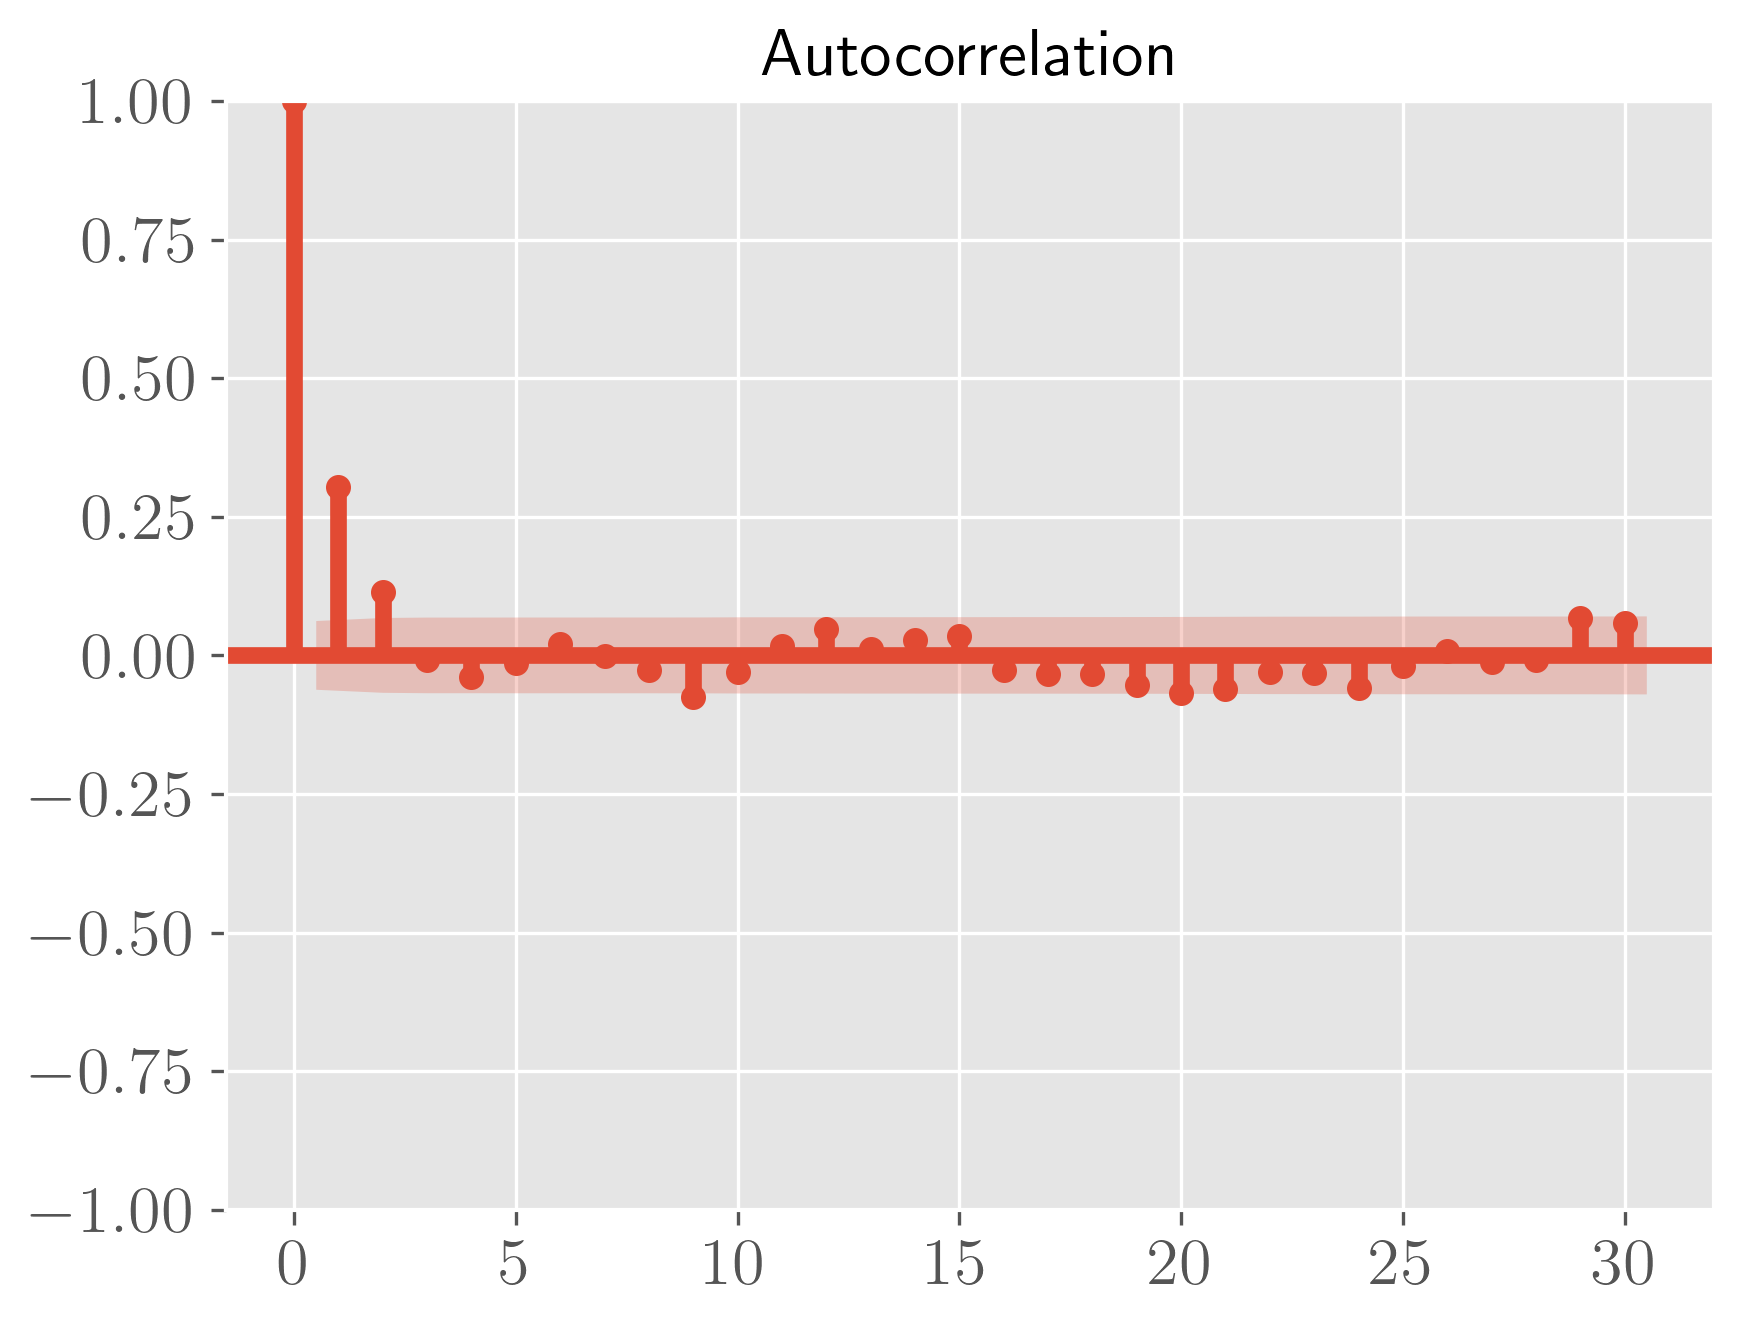
\includegraphics[scale=.6
    ]{../figures/acf2.png}
    \caption{ACF for $X_2$}
    \label{fig:my_label}
\end{figure}
\clearpage

\subsection*{(3) (a)}

\begin{align*}
    y_t &= \mu + \rho(y_{t-1} -\mu) + \epsilon_t \\
     var(y_t) &= var(\mu) + var(\rho(y_{t-1} -\mu)) + var(\epsilon_t) \\
     &= \rho^2var(y_{t-1}) + \sigma^2\\
      &= \rho^2var(y_{t}) + \sigma^2\\
      var(y_t) &= \frac{\sigma^2}{1-\rho^2}
\end{align*}

\subsection*{(b)}

Let's find the covariance between $y_t, y_{t-1}$

\begin{align*}
    cov(y_t, y_{t-1}) &= cov(\mu + \rho(y_{t-1}-\mu) + \epsilon_t, y_{t-1})\\
    &= cov(\rho y_{t-1}, y_{t-1})\\
    &= \rho var(y_{t-1})\\
    &= \rho var(y_{t})\\
\end{align*}

Then, 


\begin{align*}
    cov(y_t, y_{t-2}) &= cov(\mu + \rho(y_{t-1}-\mu) + \epsilon_t, y_{t-2})\\
    &= cov(\rho y_{t-1}, y_{t-2})\\
    &= \rho cov(y_{t}, y_{t-1})\\
    &= \rho^2 var(y_{t})\\
\end{align*}

And so on. We easily see the pattern $cov(y_t, y_{t-k}) = \rho^kvar(y_t)$, and therefore,

\begin{align*}
    corr(y_t, y_{t-k}) &= cov(y_t, y_{t-k})/[var(y_t)var(y_{t-k})]^{1/2}\\
    &=\rho^k var(y_{t}) / var(y_{t})\\
    &=\rho^k
\end{align*}

\subsection*{(c)}
\begin{align*}
    E(y_t) &= \mu + \rho E(y_{t-1}) - \mu\rho + E(\epsilon_t)\\
    &= \mu + \rho E(y_{t}) - \mu\rho\\
    E(y_t)[1-\rho] &= \mu[1-\rho]\\
    E(y_t) &= \mu
\end{align*}

Then,

\begin{align*}
    E(\bar{y}_n) &= E(\frac{1}{n}[y_1 + y_2 \ldots + y_n])\\
    &= \frac{1}{n} E([y_1 + y_2 \ldots + y_n)\\
    &= \frac{1}{n} nE(y_t)\\
    &= E(y_t) = \mu
\end{align*}



\subsection*{(d)}
\begin{align*}
var(\bar{y}_n) &= \frac{1}{n^2}var(\sum y_i)\\
&= \frac{1}{n^2}[\sum var(y_i) + 2\sum cov(y_i, y_j)]\\  
&= \frac{1}{n^2}[\sum \sigma^2/(1-\rho^2) + 2\sum   (n-j)\rho^j \sigma^2/(1-\rho^2)]\\
&= \frac{1}{n^2}\frac{\sigma^2}{1-\rho^2}[n  + 2\sum   (n-j)\rho^j] \\
\end{align*}





\subsection*{(e)} I did not have time to figure out how to prove this. So instead, I confirmed this was true with a simulation. I set $\rho = 0.75$, $\mu=0$ and $\sigma^2 = 1$. For $n$ ranging from 1 to 100,000, I calculated $nvar(\bar{y}_n)$ from the result in (d). Then, I plotted this as a function of $n$ and also plotted $\sigma^2/(1-\sigma)^2$, and the former converged to the latter as $n$ approached infinity. I attached the plot. Sorry; would be curious to see the actual answer.


\begin{figure}[!h]
    \centering
    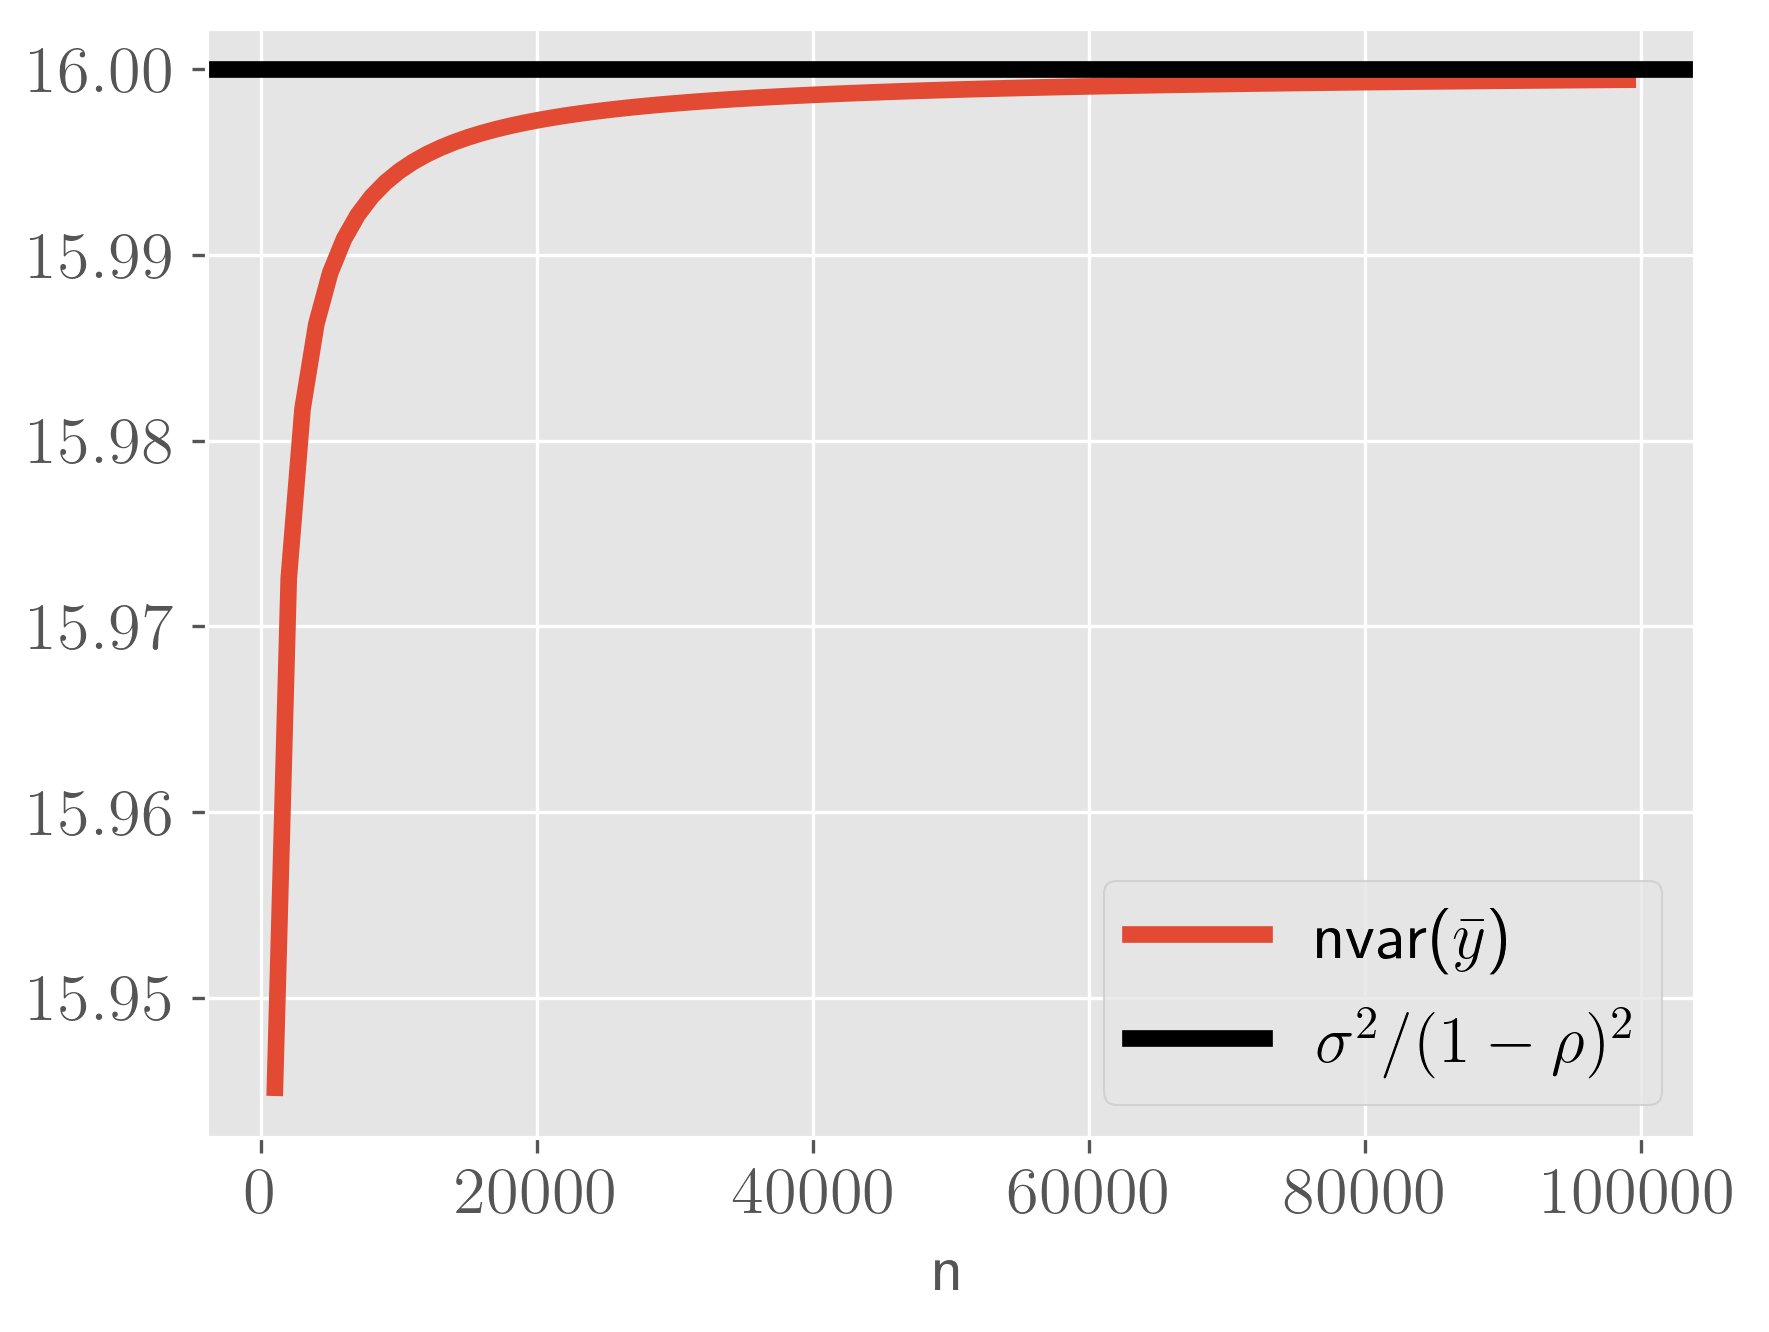
\includegraphics[scale=.5
    ]{../figures/e.png}
    \caption{``proof'' for (e)}
    \label{fig:my_label}
\end{figure}

\subsection*{(f)}
Similarly, I did not have time to figure out how to do this, so I did a quick simulation with the same parameters as for (e). I picked $n$ between 1 and 500. For each $n$, I generated $y_n$ 50 times, and calculated $s_n^2$ for each $y_n$, and took the mean of that, $E(s_n^2)$. I compared this with $var(y_t)$ from (a). The plot is shown below.  $E(s_n^2)$ seems to converge, though it is a bit noisy.

\begin{figure}[!h]
    \centering
    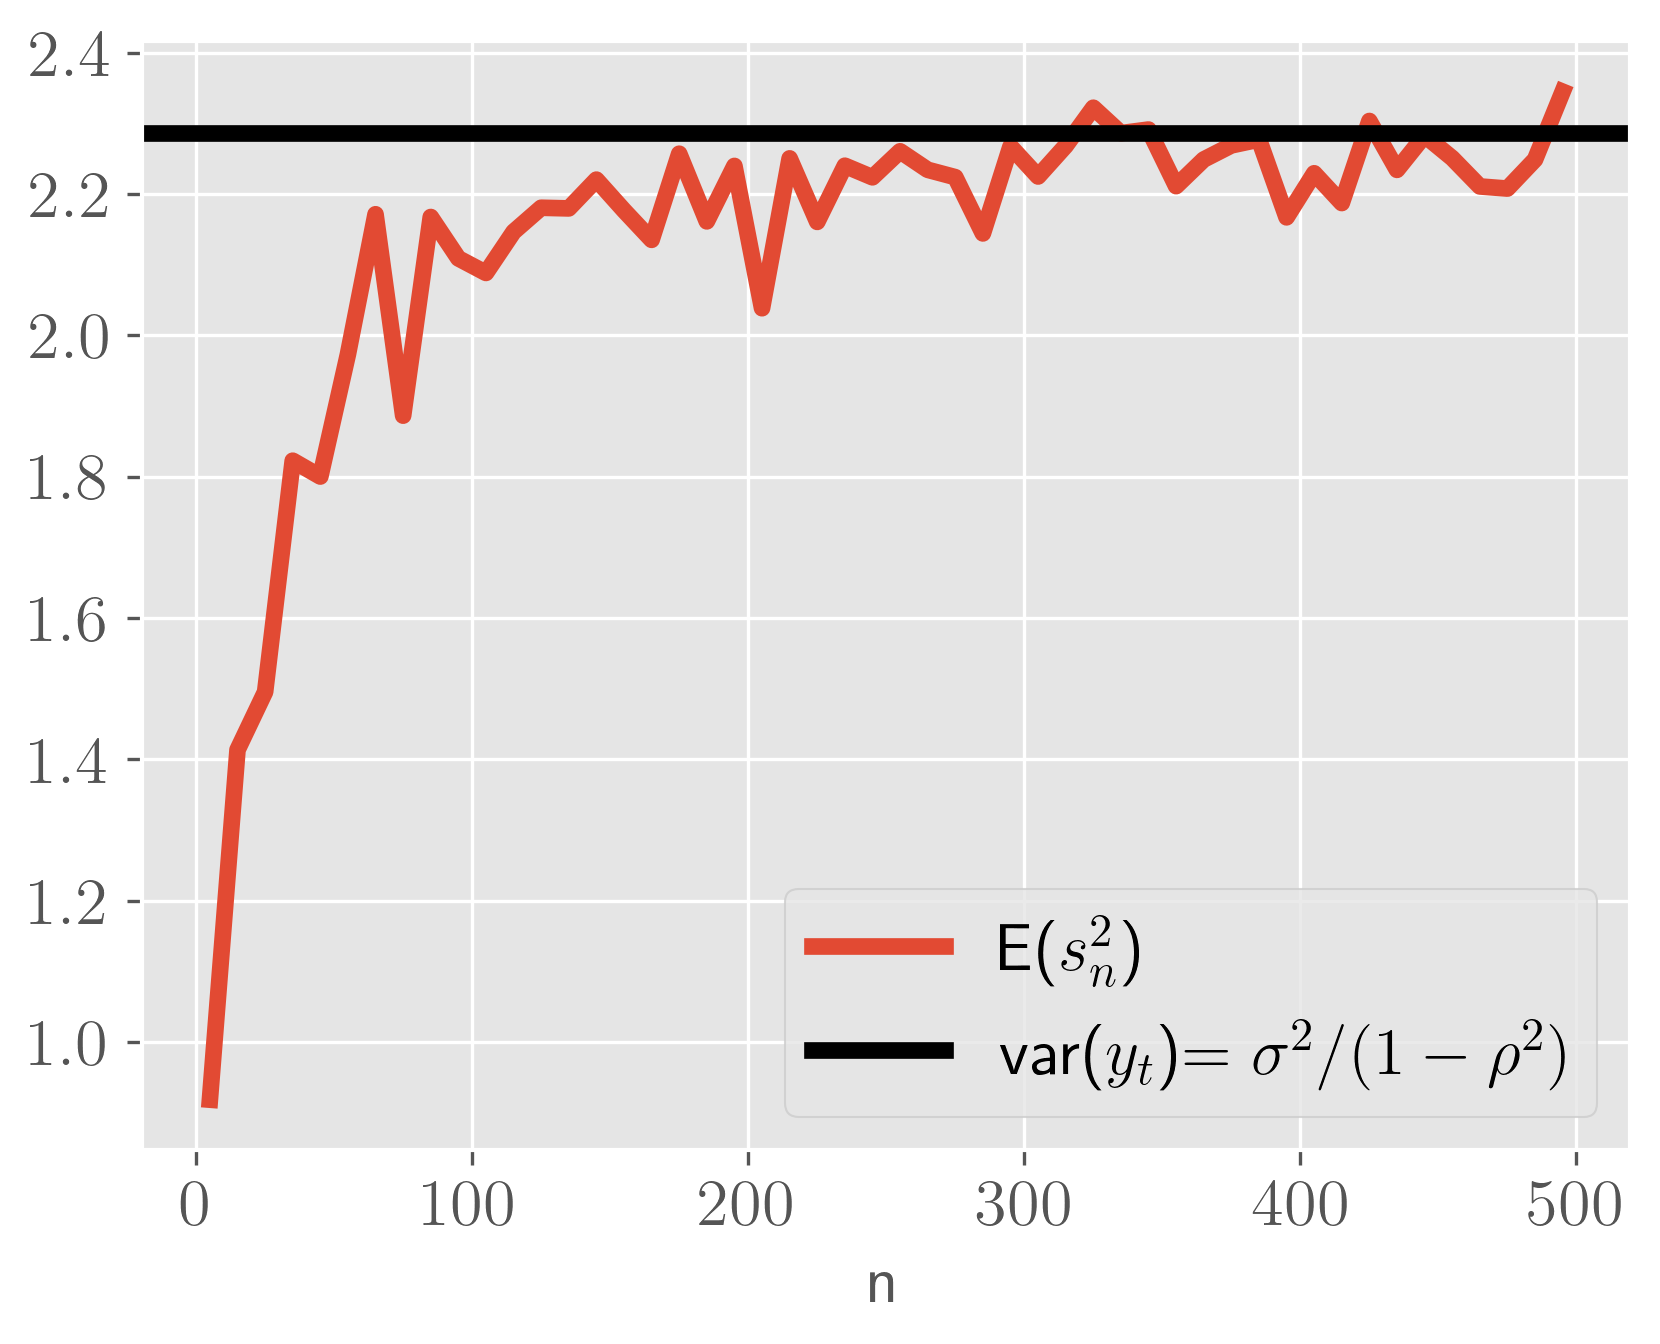
\includegraphics[scale=.5
    ]{../figures/f.png}
    \caption{``proof'' for (f)}
    \label{fig:my_label}
\end{figure}

\subsection*{(4) (a)}
I used 
\begin{align*}
    \rho & \propto \text{constant}\\
    \sigma^2 & \propto IG(\alpha, \beta)
\end{align*}

Note that I could also have used a normal on $\rho$ but this was simpler.

\subsection*{(b)}
Let us rewrite 
\begin{align*}
    y_t \sim \mathcal{N}(\rho y_{t-1}, \sigma^2)
\end{align*}
In vector form as

\begin{align*}
    \boldsymbol{y} \sim \mathcal{N}(\boldsymbol{X}\rho , \sigma^2\boldsymbol{I})
\end{align*}

Then

\begin{align*}
    p(\rho|\boldsymbol{y}, \sigma^2) &\propto p(\boldsymbol{y}|\rho)p(\rho)\\
    & \propto\text{exp} \left( -\frac{1}{2\sigma^2} \sum [y_i-X_i\rho]^2\right)\\
      & \propto\text{exp} \left( -\frac{1}{2\sigma^2} [-2\rho\sumy_iX_i + \rho^2\sum2X_i^2]\right)\\
      & \propto\text{exp} \left( -\frac{\sum X_i^2}{2\sigma^2} [-2\rho\sumy_iX_i/\sum X_i^2 + \rho^2]\right)\\
      & \propto \mathcal{N}(\sum y_i X_i / \sum X_i^2, \sigma^2/\sum X_i^2)
\end{align*}

\begin{align*}
    p(\sigma^2|\boldsymbol{y}, \rho) &\propto p(\boldsymbol{y}|\rho)p(\sigma^2)\\
    &  \propto (\sigma^2)^{-n/2}\text{exp} \left( -\frac{1}{2\sigma^2} \sum [y_i-X_i\rho]^2\right) (\sigma^2)^{-\alpha-1} \text{exp}(-\rho(\sigma^2)^{-1})\\
    &  \propto (\sigma^2)^{-n/2-\alpha-1}\text{exp} \left( -\frac{1}{\sigma^2} [0.5\sum [y_i-X_i\rho]^2 + \beta]\right)\\
    & \propto IG(\alpha + n/2, 0.5\sum [y_i-X_i\rho]^2 + \beta)
\end{align*}

\subsection*{(c)}
I chose $\alpha=\beta=0.5$

\begin{figure}[!h]
    \centering
    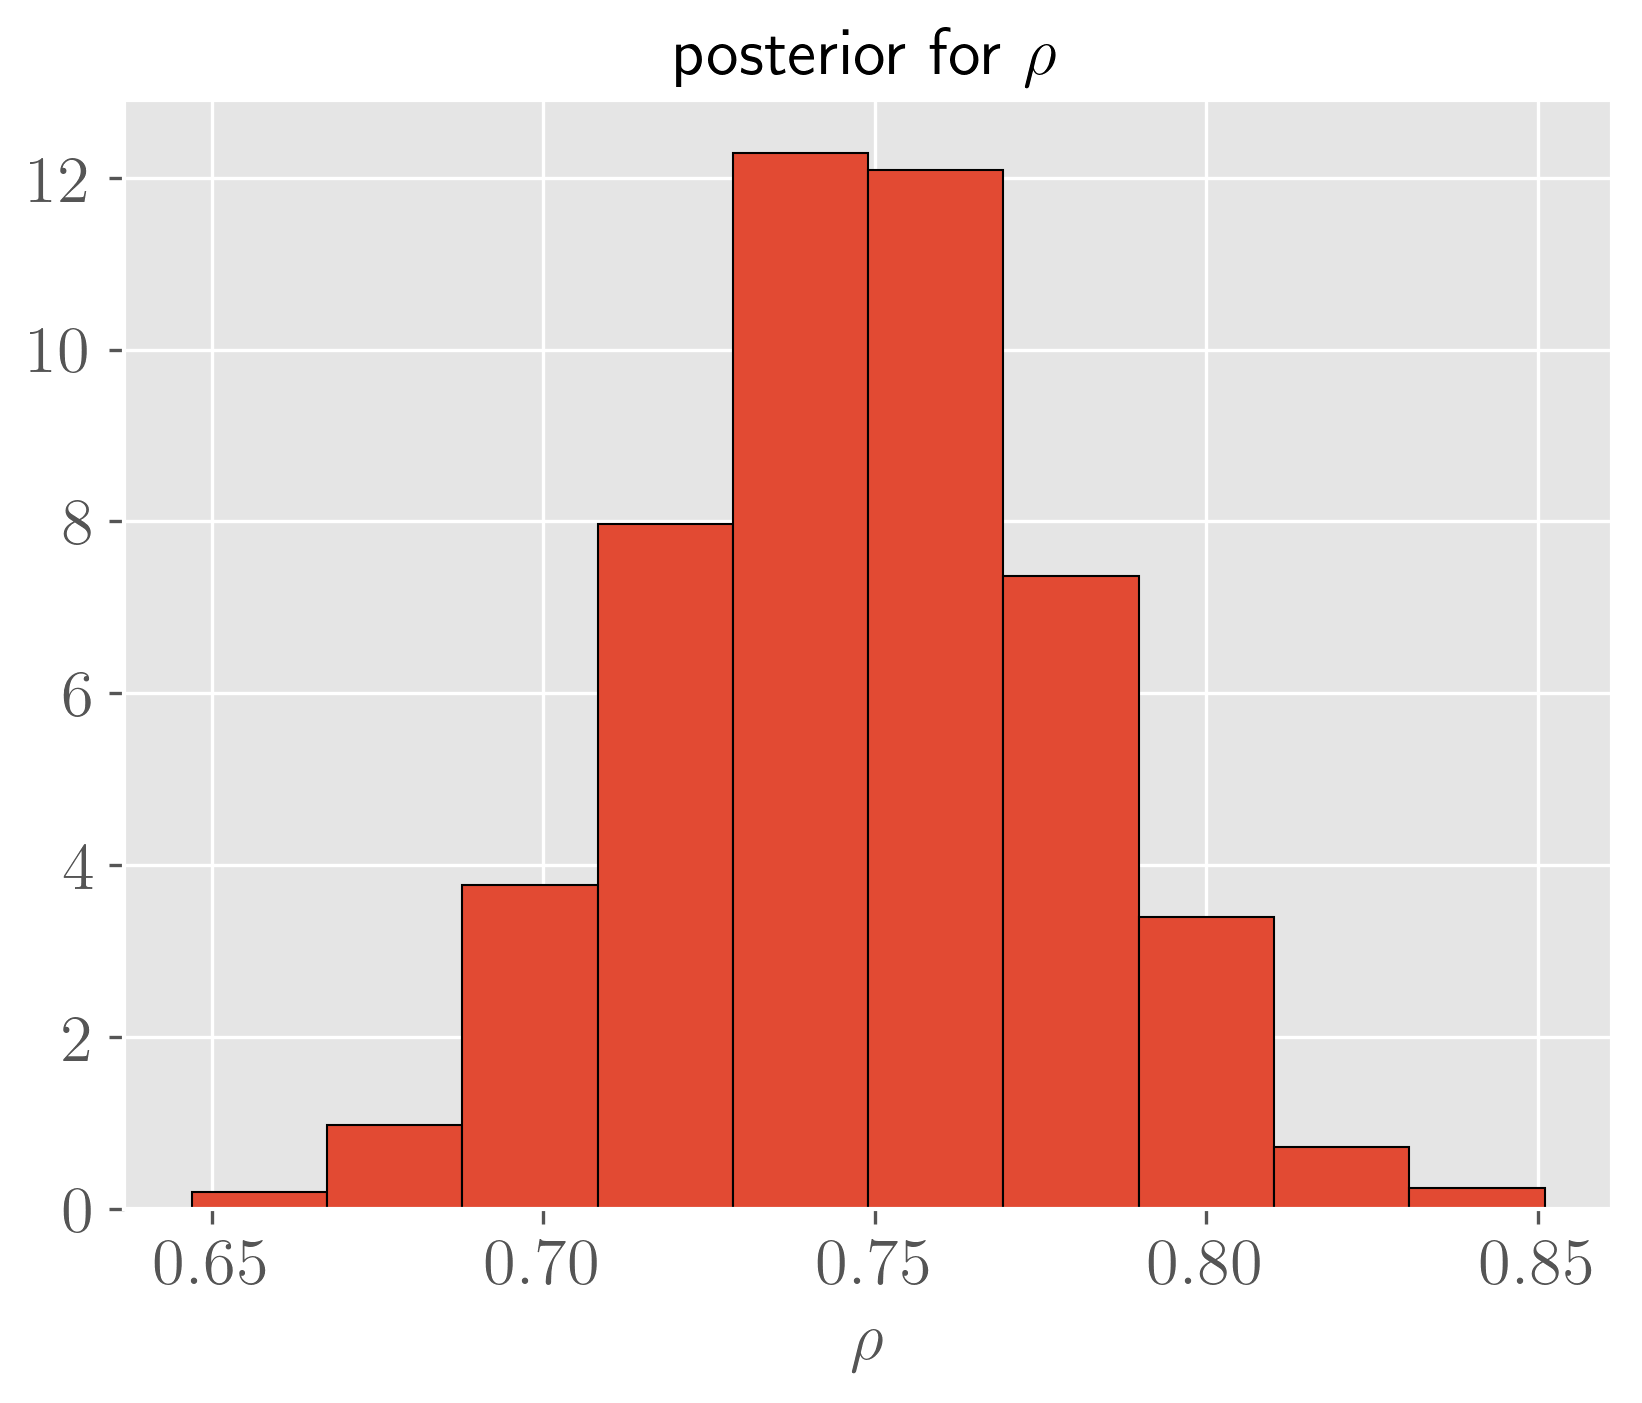
\includegraphics[scale=.6
    ]{../notebooks/rho.png}
    \caption{posterior for $\rho$}
    \label{fig:my_label}
\end{figure}

\begin{figure}[!h]
    \centering
    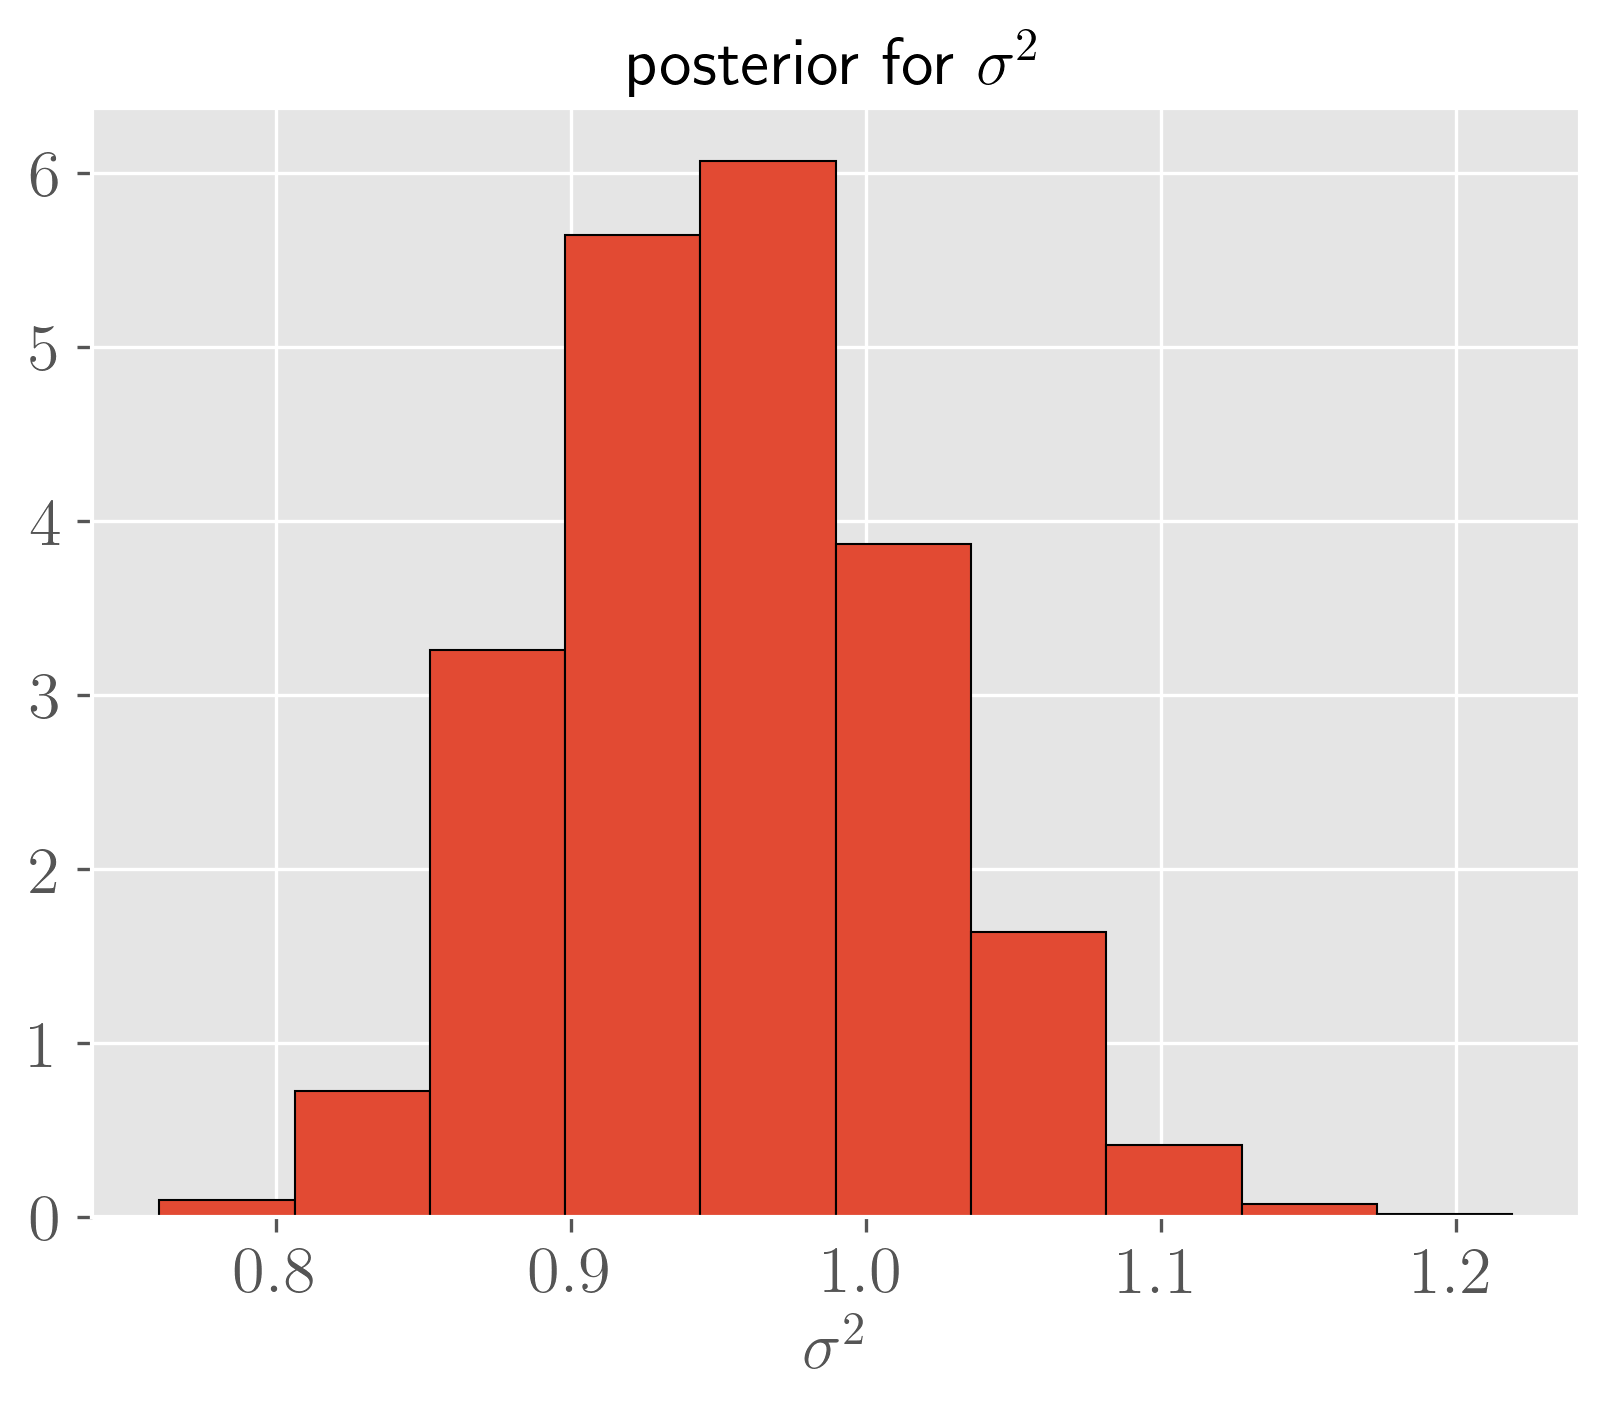
\includegraphics[scale=.6
    ]{../notebooks/sig.png}
    \caption{posterior for $\sigma^2$}
    \label{fig:my_label}
\end{figure}
\clearpage
\subsection*{(d)}
For $\rho$ [0.70, 0.80] \\
For $\sigma^2$ [0.90, 1.10] \\


\subsection*{(5)}
The general approach is:
\begin{itemize}
    \item Find full conditionals
    \item Initialize all parameters, I did this randomly 
    \item Update the parameters (2,000 iterations) by drawing from the full conditionals while recording the traces
    \item Burn and thin (burn = 500, thin = 2)
\end{itemize}

The conditionals are:

\begin{align*}
z_i &\sim mult(1, \boldsymbol{\pi}_i)\\
    \sigma_k^2 &\sim IG(\alpha + \sum 1(z_i = k)/2,  \sum 1(z_i = k)(y_i-\mu_k)^2/2 + b_0)\\
    \mu_k &\sim \mathcal{N}(\mu_k', \sigma_k^2'),  \hspace{10}  \sigma_k^2' = \frac{\sigma_k^2\sigma_0^2}{\sigma_0^2\sum 1(z_i = k) + \sigma_k^2}, \hspace{10} \mu_k = \sigma_k^2'[\sum 1(z_i = k)y_i/\sigma_k^2 + \mu_0/\sigma^2_0] \\
    \boldsymbol{w}&\sim Dir(\alpha/K + \sum 1(z_i = 1), \alpha/K + \sum 1(z_i = 2), \ldots )
\end{align*}


\begin{figure}[!h]
    \centering
    
\includegraphics[scale=.5
    ]{../figures/galaxies.png}
    \caption{Summary of results}
    \label{fig:my_label}
\end{figure}

Note: I used the same code for questions (5) and (6) given that the IW distribution with only one dimension is the same as IG. Similarly the multivariate normal in the Python package Scipy can be used even if the covariance matrix is a scalar.

\subsection*{(5)}
As before, the general approach is:
\begin{itemize}
    \item Find full conditionals
    \item Initialize all parameters, I did this randomly 
    \item Update the parameters (2,000 iterations) by drawing from the full conditionals while recording the traces
    \item Burn and thin (burn = 500, thin = 2)
\end{itemize}

The only difference is that the IG is replaced by the IW distribution and the normal update is now multi-dimensional. I derived the conditional posteriors for the multidimensional case, which look similar to those for the previous question:

\begin{align*}
z_i &\sim mult(1, \boldsymbol{\pi}_i)\\
    \boldsymbol{\Sigma_k} &\sim IW(\nu_0 + \sum 1(z_i = k),  \Psi + \Psi_0), \hspace{10} \Psi =  \sum 1(z_i = k)(X_i-\boldsymbol{\mu}_k)(X_i-\boldsymbol{\mu}_k)^T\\
    \boldsymbol{\mu}_k &\sim \mathcal{N}( \boldsymbol{\mu}_k',  \boldsymbol{\Sigma_k}'),  \hspace{10}  \boldsymbol{\Sigma_k}' = \sum 1(z_i = 1) \boldsymbol{\Sigma}_k^{-1} + \boldsymbol{\Sigma_0}^{-1}, \hspace{10} \boldsymbol{\mu}_k = \boldsymbol{\Sigma_k}'[\boldsymbol{\Sigma_k}^{-1}\sum 1(z_i = k)y_i+ \boldsymbol{\Sigma_0}^{-1}\mu_0] \\
    \boldsymbol{w}&\sim Dir(\alpha/K + \sum 1(z_i = 1), \alpha/K + \sum 1(z_i = 2), \ldots )
\end{align*}

The plot below shows the fitted posterior (mean) and the data for various Ks.

\begin{figure}[!h]
    \centering
    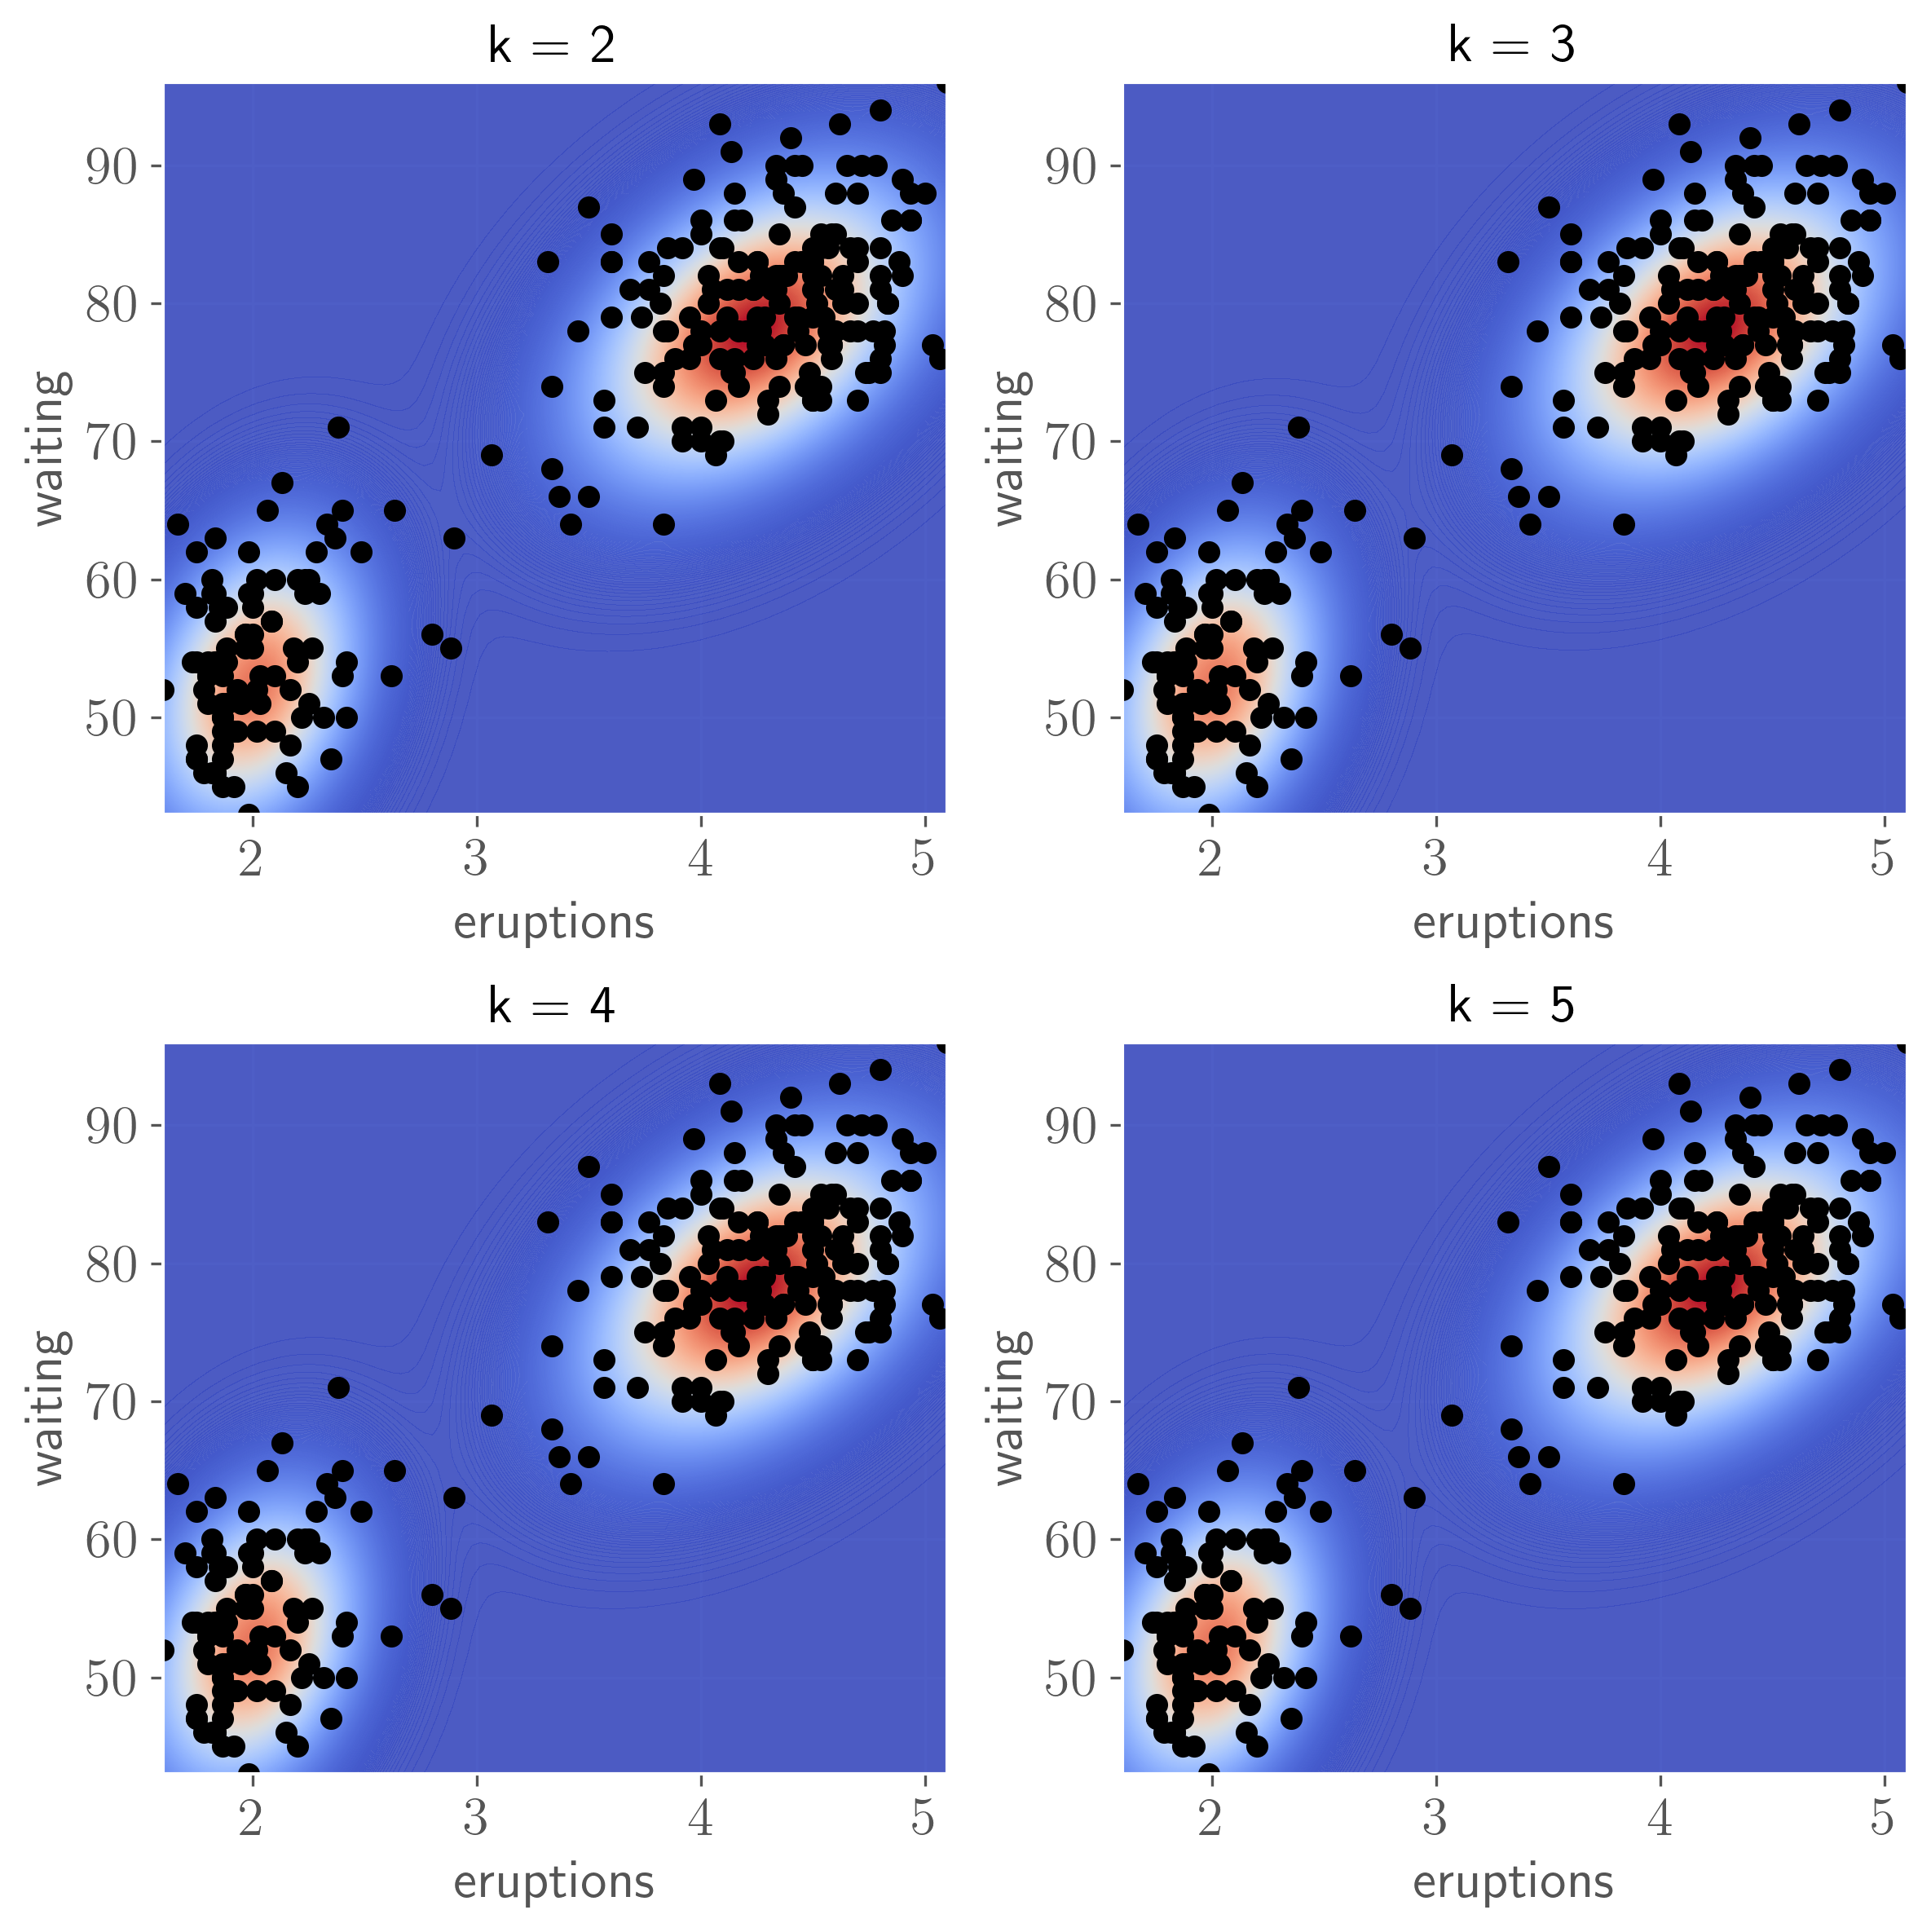
\includegraphics[scale=.6
    ]{../figures/bivariate.png}
    \caption{Summary of results}
    \label{fig:my_label}
\end{figure}

\end{document}
